\documentclass{beamer}
\usepackage{fontawesome}
\usepackage{hyperref}
\usetheme{Madrid}
\usecolortheme{sidebartab}
\usefonttheme{professionalfonts}
\urlstyle{same}

\title{Getting Started with Ansible for Network Automation}
\date{}
\author{Josh VanDeraa}

\begin{document}
% \frame{\titlepage}
\begin{frame}
  \maketitle
  \footnotesize
  \faTwitter vanderaaj \hfill \faGithub jvanderaa \hfill \faSlack jvanderaa
\end{frame}

\begin{frame}
\frametitle{Session Overview}
At the end of this session you will be able to:
\begin{itemize}
    
  \item <2-> Review the playbook management keys and values
  \begin{itemize}
    \item <3-> vars:
    \item <4-> connection:
    \item <5-> hosts:
  \end{itemize}
  \item <6-> Update an Ansible config file to manipulate playbook wide settings
  \item <7-> Gather data from various devices using command modules
    \begin{itemize}
        \item IOS
        \item NXOS
        \item Other network devices
    \end{itemize}
  \item <8-> Know where to find information about Ansible Network Modules
  \item <9-> Use regex to parse data from a command with data gathered
\end{itemize}
\end{frame}

\begin{frame}
\frametitle{Network Diagram}
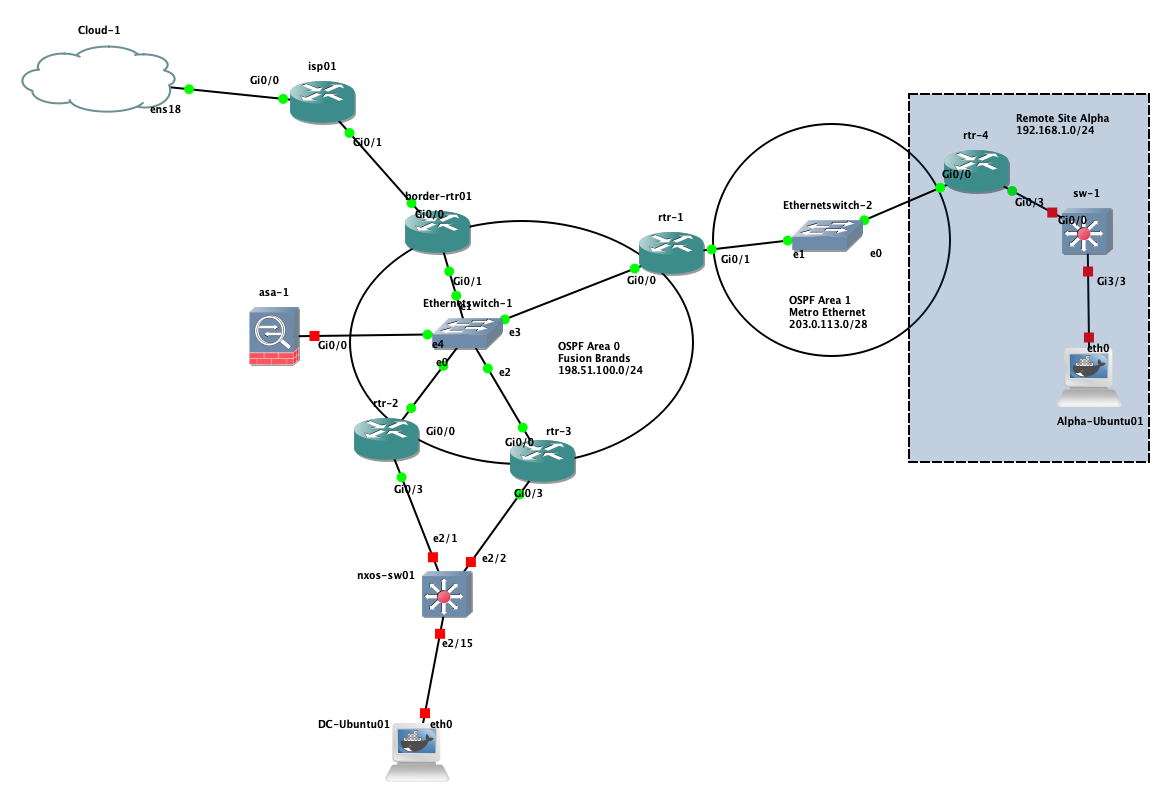
\includegraphics[width=\textwidth]{assets/base_setup.png}
\end{frame}

\begin{frame}[fragile]
    \frametitle{Playbook Management Key Values}
    All Ansible playbooks are defined within YAML format, which leverages key/value
    pair assignments. We will take a look at some common keys used, and what their
    corresponding value looks like.
\begin{verbatim}
- name: "PLAY 1: Gather data from router"
  connection: network_cli
  hosts: r1
  become: true
  become_method: enable
\end{verbatim}
\end{frame}

\begin{frame}
  \frametitle{Ansible Network Modules}
  \begin{block}{Ansible Network Modules}
    The whole list of Network modules and their corresponding requirements
    can be found with your favorite search engine on term of "Ansible Network Modules" 
    - which will take you to this link: \url{https://docs.ansible.com/ansible/latest/modules/list_of_network_modules.html}
    This will be included on the notes for this.
    \end{block}
\end{frame}

\begin{frame}
  \frametitle{Ansible Network Modules Page}
    Let's take a look at those modules
\end{frame}

\begin{frame}
    \frametitle{Gathering Data from Cisco IOS Devices}
    Today's demo: We are going to take a look at a couple of the modules used
    for gathering information from Cisco IOS devices. 
    \begin{itemize}
        \item<2-> \textbf{cli\_command}
        \item<3-> \textbf{ios\_command}
    \end{itemize}
\end{frame}

\begin{frame}
    \frametitle{ios\_command}
    \begin{itemize}
      \item <1-> This is used when working with Cisco IOS devices connecting with SSH
      \item <2-> One of the original network modules introduced with Ansible for networking devices
      \item <3-> Has evolved over time, original playbooks you will see a key \textbf{provider:} included, this is legacy
    \end{itemize}
\end{frame}

\begin{frame}
  \frametitle{DEMO!}
  \begin{columns}
  \begin{column}{0.3\textwidth}
    \Huge
    \begin{center}
      \faDesktop 
      \hspace{.5cm}
      \faRocket     
    \end{center}
  \end{column}
  \begin{column}{0.7\textwidth}
    \huge 
    Let's take a look!
    \begin{itemize}
      \item cli\_command
      \item ios\_command
    \end{itemize}
  \end{column}
\end{columns}
\end{frame}


\begin{frame}
  \frametitle{Summary}
    To review what we accomplished today:
    \begin{itemize}
      \item <1-> We reviewed the playbook management keys and values
      \item <2-> Covered how to change settings within the Ansible configs, that are helpful for Network Engineers
      \item <3-> Gathered data from IOS and NXOS devices, using multiple methods
      \item <4-> Detailed where to get more information about network modules on the Ansible documentation pages
      \item <5-> Used regex to find the number of interfaces on a device
    \end{itemize}
\end{frame}

\begin{frame}
  \frametitle{Contact}
  \huge
  You can find me and more contacts on the Packet Pushers Slack Channel. 
  \linebreak
  \begin{center}
    \normalsize
    \faSlack \hspace{.1cm}jvanderaa  
  \end{center}
  
\end{frame}

\end{document}